
%(BEGIN_QUESTION)
% Copyright 2015, Tony R. Kuphaldt, released under the Creative Commons Attribution License (v 1.0)
% This means you may do almost anything with this work of mine, so long as you give me proper credit

\noindent
{\bf Lab Exercise -- introduction}

\vskip 5pt

Your task is to build, calibrate, document, and program a temperature measurement system consisting of an electronic temperature transmitter connected to one of the analog inputs of a data acquisition module (DAQ) for a SCADA RTU (Remote Terminal Unit) node.  The particular SCADA system we will be using has been designed specifically for BTC Instrumentation students.  It is called {\sl caSCADA} and it is based on a single-board computer running the Linux operating system.  In this lab exercise you will be configuring the RTU node to receive a temperature transmitter's 4-20 mA analog signal and properly condition that data for visual display on a remote computer.  This will involve editing some of the programming code written in the ``C'' language.  Your instructor will assign the temperature to be measured, as well as the specific channel(s) to use on the caSCADA system for your loop.

The following table of objectives show what you and your team must complete within the scheduled time for this lab exercise.  Note how some of these objectives are individual, while others are for the team as a whole:

\underbar{Objective completion table:}

% No blank lines allowed between lines of an \halign structure!
% I use comments (%) instead, so that TeX doesn't choke.

$$\vbox{\offinterlineskip
\halign{\strut
\vrule \quad\hfil # \ \hfil & 
\vrule \quad\hfil # \ \hfil & 
\vrule \quad\hfil # \ \hfil & 
\vrule \quad\hfil # \ \hfil & 
\vrule \quad\hfil # \ \hfil & 
\vrule \quad\hfil # \ \hfil & 
\vrule \quad\hfil # \ \hfil \vrule \cr
\noalign{\hrule}
%
% First row
{\bf Performance objective} & {\bf Grading} & {\bf 1} & {\bf 2} & {\bf 3} & {\bf 4} & {\bf Team} \cr
%
\noalign{\hrule}
%
% Another row
Team meeting and prototype sketch (do {\it first!}) & mastery & -- & -- & -- & -- & \cr
%
\noalign{\hrule}
%
% Another row
Final wiring inspection & mastery & -- & -- & -- & -- &  \cr
%
\noalign{\hrule}
%
% Another row
T/C signal simulation ($\pm$ 1\% of span accuracy) & mastery &  &  &  &  & -- -- -- -- \cr
%
\noalign{\hrule}
%
% Another row
RTD signal simulation ($\pm$ 1\% of span accuracy) & mastery &  &  &  &  & -- -- -- -- \cr
%
\noalign{\hrule}
%
% Another row
Linux command-line usage & mastery &  &  &  &  & -- -- -- -- \cr
%
\noalign{\hrule}
%
% Another row
Editing and running caSCADA code & mastery &  &  &  &  & -- -- -- -- \cr
%
\noalign{\hrule}
%
% Another row
Lab question: Instrument connections & proportional &  &  &  &  & -- -- -- -- \cr
%
\noalign{\hrule}
%
% Another row
Lab question: Commissioning & proportional &  &  &  &  & -- -- -- -- \cr
%
\noalign{\hrule}
%
% Another row
Lab question: Mental math & proportional &  &  &  &  & -- -- -- -- \cr
%
\noalign{\hrule}
%
% Another row
Lab question: Diagnostics & proportional &  &  &  &  & -- -- -- -- \cr
%
\noalign{\hrule}
} % End of \halign 
}$$ % End of \vbox

The only ``proportional'' scoring in this activity are the lab questions, which are answered by each student individually.  A listing of potential lab questions are shown at the end of this worksheet question.  The lab questions are intended to guide your labwork as much as they are intended to measure your comprehension, and as such the instructor may ask these questions of your team day by day, rather than all at once (on a single day).

\vskip 10pt

{\bf It is essential that your team plans ahead what to accomplish each day.  A short (10 minute) team meeting at the beginning of each lab session is a good way to do this, reviewing what's already been done, what's left to do, and what assessments you should be ready for.  There is a lot of work involved with building, documenting, and troubleshooting these working instrument systems!}

As you and your team work on this system, you will invariably encounter problems.  You should always attempt to solve these problems as a team before requesting instructor assistance.  If you still require instructor assistance, write your team's color on the lab whiteboard with a brief description of what you need help on.  The instructor will meet with each team in order they appear on the whiteboard to address these problems.



\vfil \eject

\noindent
{\bf Lab Exercise -- team meeting, prototype sketch, and instrument selection}

\vskip 5pt

An important first step in completing this lab exercise is to {\bf meet with your instructor} as a team to discuss safety concerns, team performance, and specific roles for team members.  If you would like to emphasize exposure to certain equipment (e.g. use a particular type of control system, certain power tools), techniques (e.g. fabrication), or tasks to improve your skill set, this is the time to make requests of your team so that your learning during this project will be maximized.

\vskip 10pt

An absolutely essential step in completing this lab exercise is to work together as a team to {\bf sketch a prototype diagram} showing what you intend to build.  This usually takes the form of a simple electrical schematic and/or loop diagram showing all electrical connections between components, as well as any tubing or piping for fluids.  This prototype sketch need not be exhaustive in detail, but it does need to show enough detail for the instructor to determine if all components will be correctly connected for their safe function.

For example, if you intend to connect field devices to a PLC (Programmable Logic Controller), your prototype sketch must show how those devices will connect to typical input/output terminals on the PLC, where electrical power will be supplied, etc.  Prototype sketches need not show all intermediary connections between components, such as terminal blocks in junction boxes between the field device and the controller.

You should practice good problem-solving techniques when creating your prototype sketch, such as consulting equipment manuals for information on component functions and marking directions of electric current, voltage polarities, and identifying electrical sources/loads.  Use this task as an opportunity to strengthen your analytical skills!  Remember that you will be challenged in this program to do all of this on your own (during ``capstone'' assessments), so do not make the mistake of relying on your teammates to figure this out for you -- instead, treat this as a problem {\it you} must solve and compare your results with those of your teammates.

Your team's prototype sketch is so important that the instructor will demand you provide this plan before any construction on your team's working system begins.  {\it Any team found constructing their system without a verified plan will be ordered to cease construction and not resume until a prototype plan has been drafted and approved!}  Similarly, you should not deviate from the prototype design without instructor approval, to ensure nothing will be done to harm equipment by way of incorrect connections.  Each member on the team should have ready access to this plan (ideally possessing their own copy of the plan) throughout the construction process.  Prototype design sketching is a skill and a habit you should cultivate in school and take with you in your new career.

\vskip 10pt

When selecting field instruments for this project, choose an electronic temperature transmitter, either ``smart'' or analog.  The Rosemount model 644/3044/3144/3244 transmitters are good examples of smart temperature transmitters, while the Rosemount model 444 is a good example of an analog temperature transmitter.  Note that analog transmitters are built {\it either} thermocouple or RTD input.  Since you will need to calibrate {\it both} types in this lab activity, this will require two different analog transmitters!  If you choose to use a ``smart'' transmitter, however, you need only select one because digital temperature transmitters are usually configurable for both RTD and thermocouple input.

Consult documentation from the manufacturer's website to identify how to properly wire, power, and calibrate the transmitter.  Your instructor will check to see you have located and are familiar with the equipment manual(s).

After locating a suitable instrument and its associated documentation, you should qualitatively test it prior to installing it in your system.  For an analog thermocouple transmitter, you may simply short (jumper) the thermocouple input terminals to make the transmitter ``think'' it is measuring ambient temperature.  For an analog RTD transmitter, you may connect a 100 $\Omega$ resistor to the RTD input terminals to make it ``think'' it is measuring the freezing point of water.  For a digital (``smart'') transmitter, first use a HART communicator to configure it for either 2-wire RTD or thermocouple input, then proceed with these tests.  If the transmitter fails to respond properly, tag it with a label explaining what it does (or what it fails to do).

\vskip 10pt

{\bf Planning a functioning system should take no more than an hour if the team is working efficiently, and will save you hours of frustration (and possible component destruction!).}









\vfil \eject

\noindent
{\bf Lab Exercise -- building the system}

\vskip 5pt

Each RTU contains power circuitry and terminal blocks set up to marshall analog signals from field instruments to a data acquisition device.  A generic loop diagram shows how any field device may connect to the DAQ.  Your final loop diagram will simply be a customized version of this generic diagram provided to you near the end of this worksheet.

Each loop has a pre-assigned loop number, kept on file by the instructor to ensure each loop is uniquely labeled.  Your transmitter and its signal wiring should be labeled with the loop number to distinguish it from other loops.

\vskip 10pt

{\bf Common mistakes:}

\begin{itemize}
\item{} Neglecting to consult the manufacturer's documentation for field instruments (e.g. how to wire them, how to calibrate them).
\item{} Mounting the field instrument(s) in awkward positions, making it difficult to reach connection terminals or to remove covers when installed.
\item{} Failing to tug on each and every wire where it terminates to ensure a mechanically sound connection.
\item{} Students working on portions of the system in isolation, not sharing with their teammates what they did and how.  It is important that the whole team learns all aspects of their system!
\end{itemize}

\vskip 10pt

{\bf Building a functioning system should take no more than one full lab session (3 hours) if all components are readily available and the team is working efficiently!}







\vfil \eject

\noindent
{\bf Lab Exercise -- instrument calibration and signal simulation}

\vskip 5pt

Each team must calibrate the transmitter to ensure it interprets temperature accurately and outputs an accurate current, and also scale the SCADA system channel to register in the proper engineering units (e.g. a temperature transmitter ranged for 0 to 200 degrees F should actually register 0 to 200 deg F back at the SCADA system display).  Instructions for programming the caSCADA system with the proper range for your measurement loop are explained later in this document.  Each team should choose a temperature range that covers room temperature, but is something {\it other} than 0 to 100 degrees so they get practice setting range points on the controller to values other than the default (0 to 100\%).  Teams using a ``smart'' temperature transmitter may need to ``trim'' both the input and output of their transmitter, then set the range (LRV and URV points).  Teams using an analog transmitter must apply LRV and URV electrical signals to the transmitter's input while adjusting the ``zero'' and ``span'' potentiometers on the transmitter.

As in all cases where an instrument must be calibrated, you will need to check the instrument's response against one or more {\it standards}.  In this case, the standard we will use is either millivoltage (thermocouple) or resistance (RTD) applied to the input of the temperature transmitter using a thermocouple/RTD simulator, while we use a multimeter to measure the transmitter's electronic output signal in DC milliamps:

$$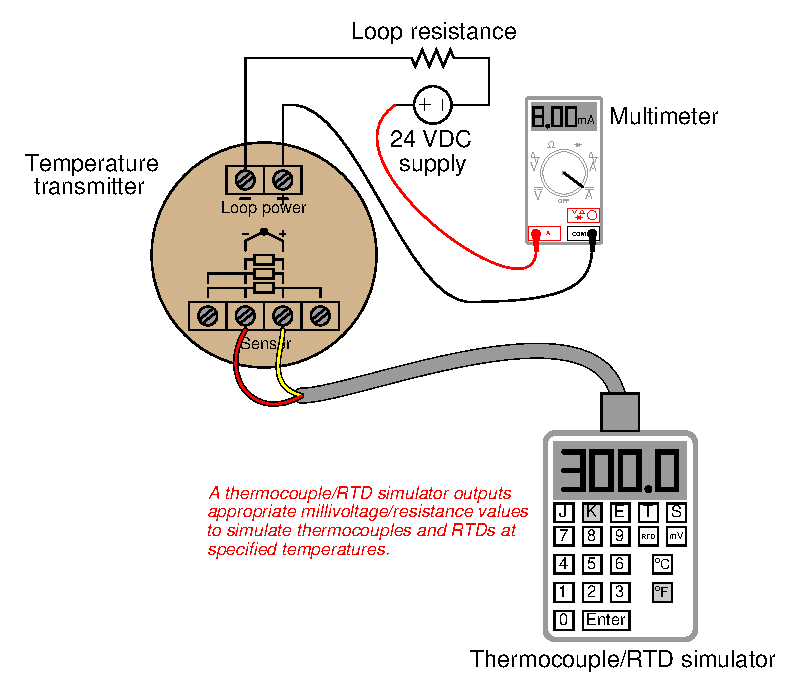
\includegraphics[width=15.5cm]{i03866x01.eps}$$

This calibration may be performed at the calibration bench or other work-table, or in the field.  Refer to the simulator's documentation for more information on how to make proper wire connections to the transmitter being calibrated.  This is especially helpful when simulating 3- or 4-wire RTD sensors.

\filbreak

Document the accuracy of your transmitter's sensor trim before and after adjustment in this table, at five different points throughout its sensing range using these two tables:

\vskip 10pt

{\bf As-Found calibration table}

% No blank lines allowed between lines of an \halign structure!
% I use comments (%) instead, so that TeX doesn't choke.

$$\vbox{\offinterlineskip
\halign{\strut
\vrule \quad\hfil # \ \hfil & 
\vrule \quad\hfil # \ \hfil & 
\vrule \quad\hfil # \ \hfil & 
\vrule \quad\hfil # \ \hfil \vrule \cr
\noalign{\hrule}
%
% First row
Applied temperature & Output signal (actual) & Output signal (ideal) & Error (\% of span) \cr
%
\noalign{\hrule}
%
% Another row
 &  &  & \cr
%
\noalign{\hrule}
%
% Another row
 &  &  & \cr
%
\noalign{\hrule}
%
% Another row
 &  &  & \cr
%
\noalign{\hrule}
%
% Another row
 &  &  & \cr
%
\noalign{\hrule}
%
% Another row
 &  &  & \cr
%
\noalign{\hrule}
} % End of \halign 
}$$ % End of \vbox

\vskip 10pt

{\bf As-Left calibration table}

% No blank lines allowed between lines of an \halign structure!
% I use comments (%) instead, so that TeX doesn't choke.

$$\vbox{\offinterlineskip
\halign{\strut
\vrule \quad\hfil # \ \hfil & 
\vrule \quad\hfil # \ \hfil & 
\vrule \quad\hfil # \ \hfil & 
\vrule \quad\hfil # \ \hfil \vrule \cr
\noalign{\hrule}
%
% First row
Applied temperature & Output signal (actual) & Output signal (ideal) & Error (\% of span) \cr
%
\noalign{\hrule}
%
% Another row
 &  &  & \cr
%
\noalign{\hrule}
%
% Another row
 &  &  & \cr
%
\noalign{\hrule}
%
% Another row
 &  &  & \cr
%
\noalign{\hrule}
%
% Another row
 &  &  & \cr
%
\noalign{\hrule}
%
% Another row
 &  &  & \cr
%
\noalign{\hrule}
} % End of \halign 
}$$ % End of \vbox

When finished calibrating your team's transmitter, be sure to place a calibration tag on it showing the range and the date it was calibrated.  A set of calibration tags are shown here which you may cut out and tape to the transmitter after completing your calibration:

$$\includegraphics[width=15.5cm]{i03866x17.eps}$$

\vskip 10pt

After each team calibrates their transmitter and installs it in the working system, each student on the team must then individually demonstrate their understanding of the electrical signals generated by thermocouples and RTDs by manually simulating appropriate signals at the input of the transmitter to make it register random temperatures called out by the instructor.  The purpose of doing this is to ensure each student understands how thermocouples and RTDs actually work, and are familiar with the purpose and use of thermocouple and RTD tables. 

For example, if a team calibrates and installs a type J thermocouple transmitter with a range of 0 to 150 degrees Fahrenheit, the instructor will choose a different temperature value within that range (e.g. 102, 93, 77, 128 $^{o}$F) for each student on the team to simulate using simple electrical equipment (no thermocouple/RTD simulators allowed here!).  Each student passes the ``T/C signal simulation'' objective when they are able to successfully simulate a specified temperature using nothing more than a multimeter and a low-voltage source (e.g. a DC power supply connected to a voltage divider circuit).  Each student passes the ``RTD signal simulation'' objective when they are able to successfully simulate a specified temperature using nothing more than a multimeter and a low-range variable resistance (e.g. a potentiometer, or a decade resistance box).  The instructor checks to see that the temperature value specified appears on the SCADA system display to within $\pm$ 1\% of transmitter span.

\filbreak

The following illustrations show the general scheme of thermocouple (``T/C'') and RTD signal simulation.  Resistor values shown in these illustrations are examples only, and may need to be modified for your particular application.  {\it Invest the necessary time for all team members to thoroughly understand how and why these potentiometer networks function as thermocouple and RTD simulators}:

$$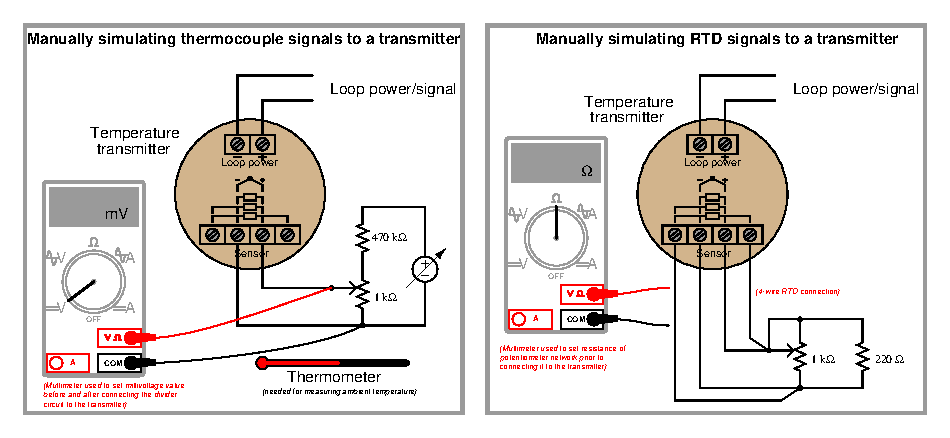
\includegraphics[width=15.5cm]{i03866x02.eps}$$

It is recommended that you use a terminal strip rather than a solderless ``breadboard'' to construct your potentiometer networks, due to the unstable contact resistance typical of breadboards.  Use the ``relative'' function on your DMM's resistance scale to ``zero out'' the electrical resistance of your meter's test leads when using it to set the resistance of your RTD-simulating network.  If your DMM supports a ``high resolution'' mode for millivoltage measurement, you should use that mode when setting the voltage signal of your thermocouple-simulating network.

Students typically find the accurate simulation of thermocouple signals to be more challenging than RTD signals, since RTDs simply manifest a certain amount of resistance at each temperature, while thermocouple signals vary with the process (measured) temperature {\it and} the ambient temperature at the transmitter terminals.  For more information on the simulation of thermocouple signals, refer to the ``Thermocouples'' section of the ``Continuous Temperature Measurement'' chapter of {\it Lessons In Industrial Instrumentation}.

\vskip 10pt

{\bf Common mistakes:}

\begin{itemize}
\item{} Applying excessive voltage to the input of a thermocouple or RTD transmitter.  Remember that thermocouples only output small amounts of voltage, in the low millivolt range.  I have seen students {\bf destroy} thermocouple transmitters by applying as little as 1.5 volts to its input terminals, thinking that would be a safe amount of voltage for the transmitter!!!  To avoid this mistake, set the millivolt signal of your simulating circuit {\it before} connecting it to the input of your transmitter.
\item{} Neglecting to accurately measure the ambient temperature when manually simulating a thermocouple signal (in order to look up the correct reference junction millivoltage).
\item{} Mis-interpreting rows and columns in the thermocouple/RTD table when looking up millivoltage or resistance values.
\item{} Choosing a calibration (``trim'') range that is substantially less than the final range of measurement when installed.  As a general rule, you should trim the sensor of the transmitter to cover the broadest range of measurement possible with your calibration equipment.
\item{} Neglecting to place a calibration tag on the transmitter after calibrating it.
\end{itemize}

\vskip 10pt

{\bf Calibrating your team's transmitter should take no more than one full lab session (3 hours) if the team is working efficiently!}








\vfil \eject

\noindent
{\bf Remote administration using SSH}

\vskip 5pt

When the Raspberry Pi computer is working to gather data from field instruments, it will be located in a water-tight enclosure without convenient physical access.  Attaching a keyboard and monitor to it will be impractical.  Therefore, you will need to log in through some other means.

Fortunately, a digital communication protocol has been developed to permit remote access of Linux operating systems called {\it SSH}, which stands for {\it Secure SHell}.  Any computer running an SSH client program is able to log into any Linux computer running an SSH server program, which the Raspberry Pi computers conveniently provide.

One such SSH client made for Microsoft Windows operating systems is called {\tt Bitvise}.  Another one is called {\tt PuTTY}.  For the really ambitious there is even a complete Linux terminal emulation package for Microsoft Windows called {\tt Cygwin}.  Any of these programs will suffice, but the easiest to download, install, and use is {\tt Bitvise}.  Be sure you download and install the {\it client} software for {\tt Bitvise}, and not the {\it server} software (which is already installed and running on the Raspberry Pi Linux computer)!

\vskip 10pt

The following screenshot shows {\tt Bitvise} running on a Windows XP machine, communicating with a Raspberry Pi computer:

$$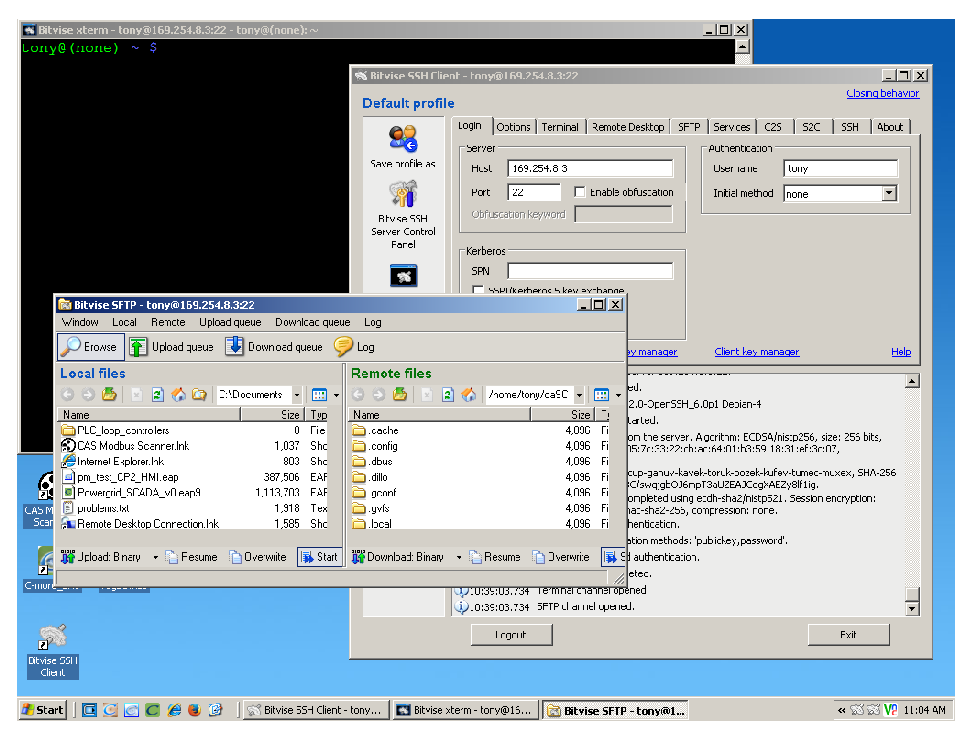
\includegraphics[width=15.5cm]{i03866x14.eps}$$

Three windows appear in this screenshot: the {\tt Bitvise} client through which the login connection is established (you must enter the Raspberry Pi's IP address and Linux user name, then later enter the Linux password for that user account), the {\tt Bitvise} SFTP window for file transfer between the two computers, and the {\tt xterm} terminal window (the one with the black background and colorful prompt) where you may enter typed commands to the Raspberry Pi computer.  Since Linux is a multi-user operating system, many people can log into the Raspberry Pi using their own individual Windows PCs, even under the same user name!  All you need is a network connection to the Raspberry Pi and its IP network address.








\vfil \eject

\noindent
{\bf Linux command-line usage}

\vskip 5pt

The caSCADA telemetry system is built on the foundation of a single-board computer called a ``Raspberry Pi'' running the Linux operating system.  Linux is a very robust alternative to Microsoft Windows, and it happens to be entirely free.  To use this operating system, you will need to become familiar with typing text-based commands into a {\it command-line interface} and reading the results given back to you by the computer, rather than pointing and clicking with a mouse.  Linux does support mouse-based user interfaces, but the text-based interface is more efficient from the perspective of processing power and memory and so it is what we will use here.

\vskip 10pt

If you have ever used the {\tt cmd} (``command'') window on a Microsoft operating system to run utilities such as {\tt ping} or {\tt ipconfig} for network troubleshooting, you are already familiar with what a command-line interface is.  Here is an example of the Linux command {\tt ifconfig} (similar to the Windows command {\tt ipconfig}) being run in the command-line interface:

$$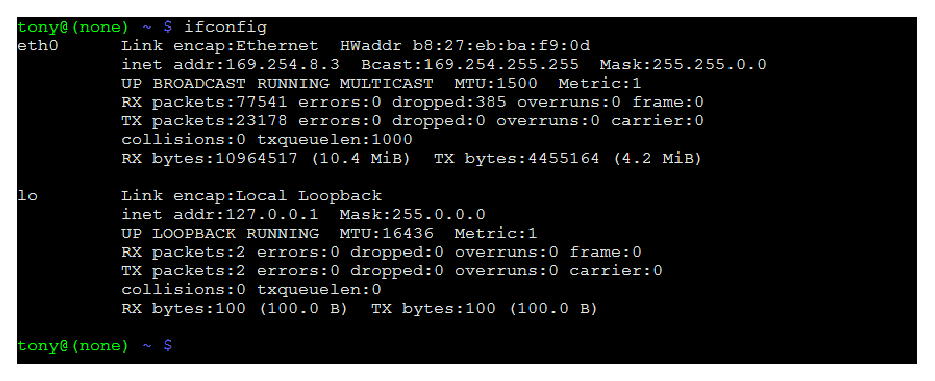
\includegraphics[width=15.5cm]{i03866x03.eps}$$

The dark blue text ({\tt \~{} \$}) is called the {\it prompt}, which shows me which directory on the computer's filesystem I'm currently viewing and working under.  The green text to the left of the prompt tells me I'm logged into the Linux operating system under the username {\tt tony} with an undefined domain name.  In a fully configured system, the domain might be something like {\tt btc.edu} or {\tt RTU\_MC1}.  The white text {\tt ifconfig} is the command I typed (pressing the Enter key at the end), and the two ``paragraphs'' of text following that line are the results of running the {\tt ifconfig} command.  In this particular example it tells me details about the two network interfaces operational on this computer: one ethernet interface ({\tt eth0}) and one called a ``loopback'' ({\tt lo}).

\vskip 10pt

There are a great multitude of typed commands available within the command-line environment of the Linux operating system.  We will only need to use a few to do our work with the caSCADA system.  The next several pages showcase those commands you should learn in order of their importance.


\vfil \eject

\vbox{\hrule \hbox{\strut \vrule{} {\tt ls} \vrule} \hrule} 

The {\tt ls} command lists the contents of a directory, or folder, on the computer's filesystem.  Here is an example of the {\tt ls} command being issued by myself ({\tt tony}) while working in my ``home'' directory ({\tt /home/tony} which is abbreviated as {\tt \~{}}):

$$
\includegraphics[width=15.5cm]{i03866x04.eps}$$

The two dark blue listings ({\tt caSCADA} and {\tt Desktop}) are both directories within my home directory (called ``subdirectories'').  Think of these as folders in which we may store files.  The white listing ({\tt letter.txt}) is a file.  The light blue listing ({\tt pistore.desktop}) is a {\it link} to a file of the same name located in a completely different directory.  In the Microsoft Windows world, a link is called a {\it shortcut}.

\vskip 20pt

\vbox{\hrule \hbox{\strut \vrule{} {\tt ls -l} \vrule} \hrule} 

This is the same command, issued with the {\tt -l} option.  Many Linux commands have options you may specify, each one preceded by a dash.  In this case, the {\tt -l} option instructs the {\tt ls} command to provide a {\it long} (i.e. more detailed) listing of the same files and directories.  It should be noted that the {\tt l} symbol is a lower-case letter L, and not the number 1.
 
$$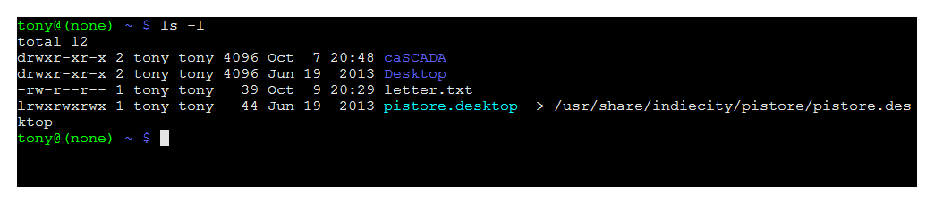
\includegraphics[width=15.5cm]{i03866x05.eps}$$

Here we see how the ``long'' listing provides much more detail.  The series of 10 characters starting each line tell us what type of listing each line is and who has permission to use it ({\tt d} for {\it directory}, {\tt l} for {\it link}, a dash symbol for regular files, {\tt w} for {\it write} permission, {\tt r} for {\it read} permission, and {\tt x} for {\it executable} permission).  We can also tell the owner and group of each listing ({\tt tony}), the size of the file in {\it bytes}, and the last date and time that listing was changed.

You will use the {\tt ls} and {\tt ls -l} commands frequently to see which files and directories are accessible to you.



\vfil \eject

\vbox{\hrule \hbox{\strut \vrule{} {\tt cd} \vrule} \hrule} 

The {\tt cd} (``change directory'') command moves you from one directory to another.  This is analogous to clicking on folder symbols in a Microsoft Windows environment.  Here we see the {\tt ls} command issued to list all the items in my home directory ({\tt \~{}}), then the {\tt cd} command issued to descend into the {\tt caSCADA} directory, then the {\tt ls} command issued one more time to list all the files contained in the {\tt caSCADA} directory:

$$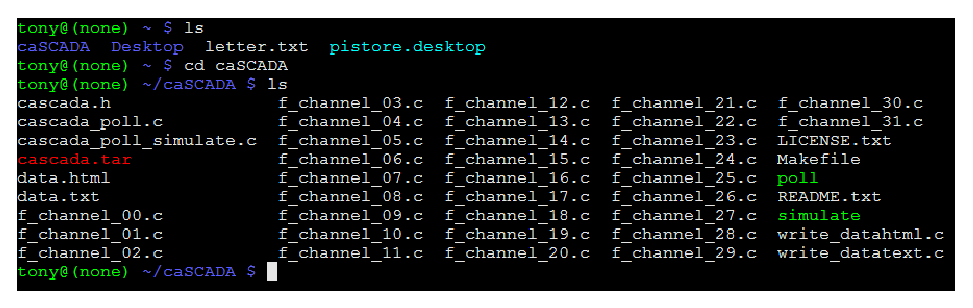
\includegraphics[width=15.5cm]{i03866x06.eps}$$

Note how the dark blue prompt changed from {\tt \~{}} to {\tt \~{}/caSCADA} after issuing the {\tt cd} command.  This is a reminder to you, the user, of which directory you are currently ``in'' as you do your work in the command-line environment.

\vskip 10pt

If we wish to go back up one directory level, we invoke the commmand {\tt cd ../} and it will take you there.  If you wish to return to your home directory, simply invoke {\tt cd} without any options or arguments and you will go back home regardless of your present location.



\vfil \eject

\vbox{\hrule \hbox{\strut \vrule{} {\tt nano} \vrule} \hrule} 

One of the most important applications you will use when using Linux is a {\it text editor}, used to create and modify plain-text files.  You may think of a text editor as being a kind of simplified word processor because it doesn't offer any means of formatting the text to look nice on paper.  However, text editors are powerful tools for programming because (most of them) offer {\it syntax-sensitive coloring} to render certain programming instructions in different colors to make them easier to identify.

{\tt nano} is a popular text editor found on practically all Linux operating systems.  It is fast and easy to learn, which is why I'm recommending it to you.  To start this program, simply type {\tt nano} at the command prompt and you will get a mostly blank screen with some key-command reminders at the bottom, like this:

$$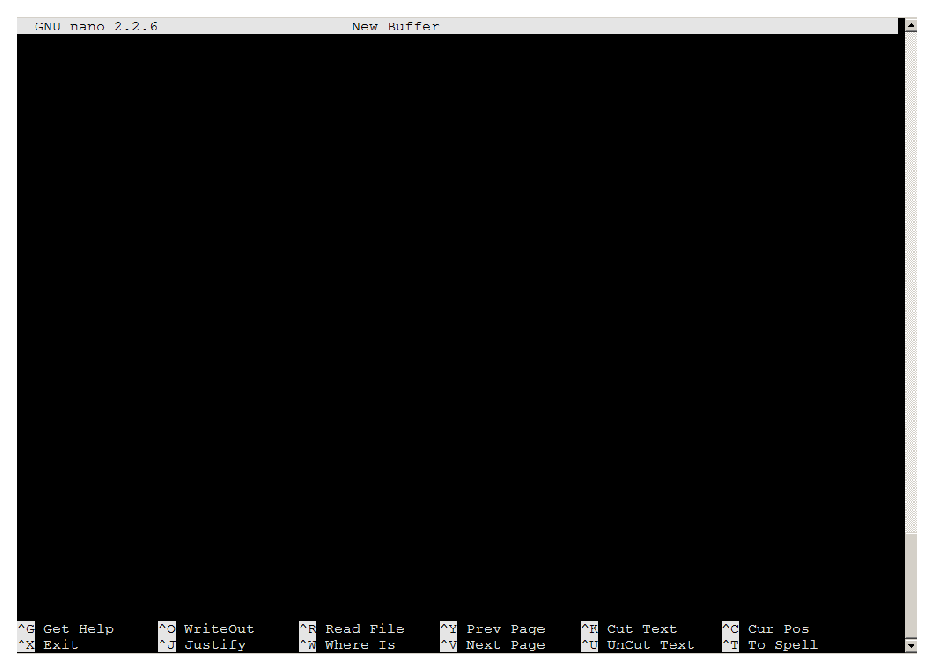
\includegraphics[width=15.5cm]{i03866x07.eps}$$

Most of the screen is blank because {\tt nano} hasn't been told to open any file, and therefore there is no content to view.  This is like starting up Microsoft Word (a heinous monstrosity of a program) with a blank page, before we have typed anything.  The inverse-colored symbols at the bottom of the screen show you common {\tt nano} commands, such as viewing a help menu ({\tt \^{}G} which means holding the ``Ctrl'' key down while pressing the ``G'' key), or writing your edits to a file ({\tt \^{}O}), or exiting the {\tt nano} text editor ({\tt \^{}X}) entirely.


\vfil \eject

If we wish to use {\tt nano} to edit a particular file within our current directory instead, we would simply type {\tt nano} at the prompt followed by the name of the file we wish to edit.  Here we see the results of typing {\tt nano f\_channel\_00.c} at the command-line prompt:

$$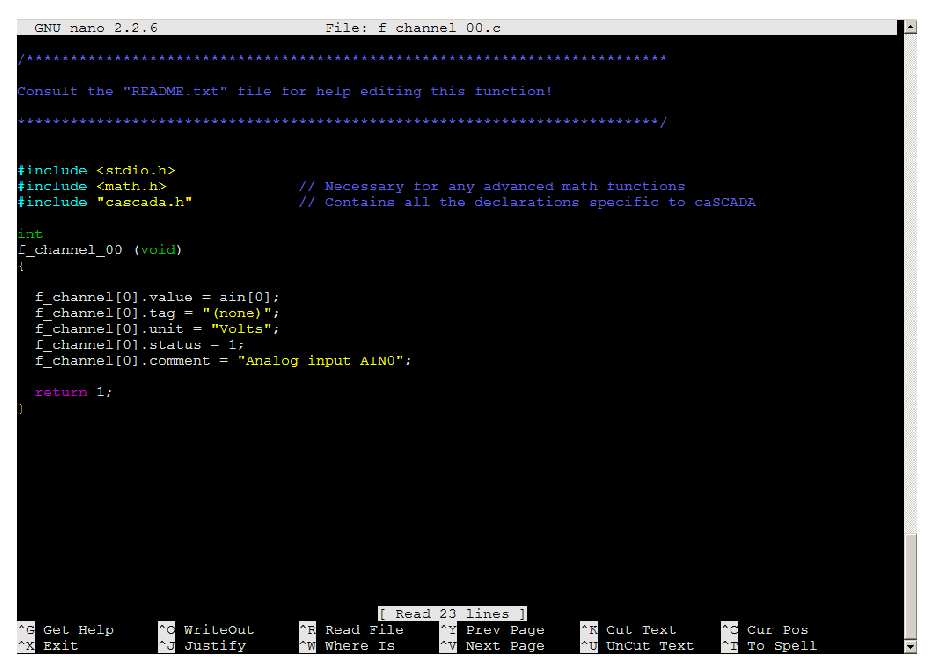
\includegraphics[width=15.5cm]{i03866x08.eps}$$

The file named {\tt f\_channel\_00.c} is one of the files containing programming code to instruct the caSCADA system what to do.  This particular file controls the information for channel 0 in the caSCADA system.  You will be editing a source file much like this one when you do your configuration work for the caSCADA system, just for a different channel number.  The various colors rendered by {\tt nano} as it views the contents of this file have different meanings in the {\it C} programming language, and make the code easier to comprehend than if it were all shown in white.  

Once you are viewing the contents of a file, you may use the arrow keys, page up/down keys, Enter key, Delete key, Backspace key, and all the alpha-numeric keys on your keyboard to write and edit text into this file.  When complete, you use the command Ctrl-X to save and exit from {\tt nano}.



\vfil \eject

\vbox{\hrule \hbox{\strut \vrule{} {\tt cat} \vrule} \hrule} 

The {\it concatenate} command, abbreviated {\tt cat}, simply reads the contents of a text file and prints it all to the screen in the command-line environment.  In this example we see the {\tt cat} command used to print the contents of a file named {\tt data.txt} residing within the {\tt caSCADA} directory we have navigated to:

$$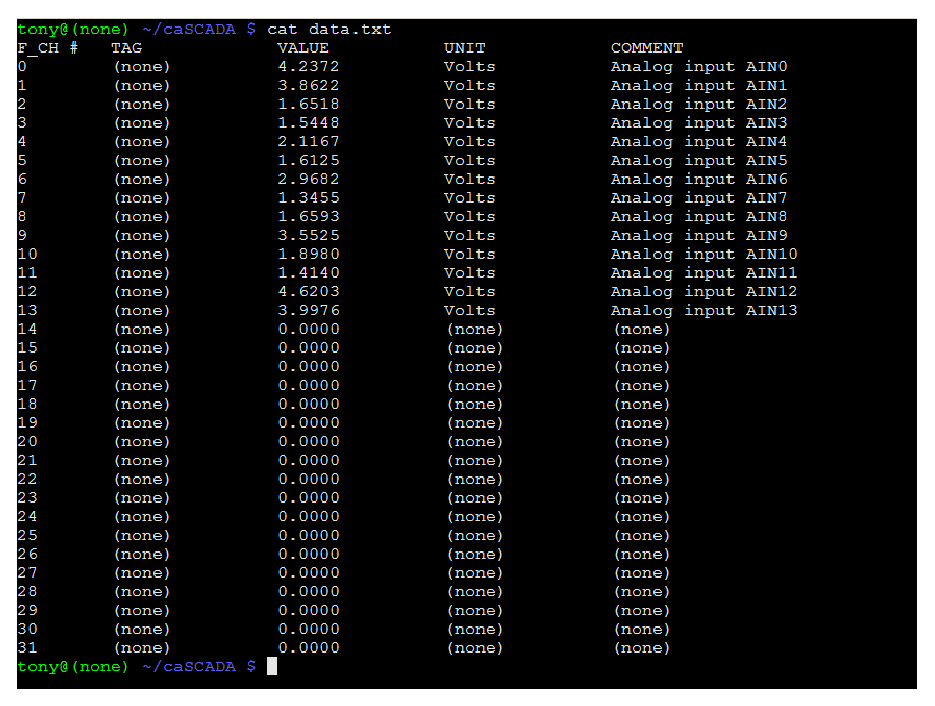
\includegraphics[width=15.5cm]{i03866x09.eps}$$

We could have easily viewed the contents of the {\tt data.txt} file using a text editor program such as {\tt nano}, but {\tt cat} is faster and more convenient if all we want to do is {\it look} at what the file contains and not edit (change) it.

\vskip 10pt

If you choose to learn more about the Linux, you will find that a great many details of the operating system are represented by and controlled by plain-text files.  Knowing how to edit those files with a text editor and view those files using {\tt cat} are nothing less than survival skills for Linux users.

\vskip 10pt

Using the {\tt cat} command to display the contents of the {\tt data.txt} file is something you will undoubtedly find yourself doing as you work with the caSCADA system: this file happens to show all the conditioned data in the caSCADA system.  As you can see here, the {\tt data.txt} file shows us the last-recorded view of all analog input voltages being read by the data acquisition unit (DAQ), and later when we've customized the C programming code for our instrument loops this same file will show us the signals scaled and presented as real-world measurements.




\vfil \eject

\vbox{\hrule \hbox{\strut \vrule{} {\tt who} \vrule} \hrule} 

Linux is a {\it multi-user} operating system, which means multiple people may log into one computer at any given time, either with individual login names or even under the same name!  Microsoft Windows, by contrast, was designed to support only one user at a time.  The {\tt who} command gives a listing of all the users logged into the Linux operating system:

$$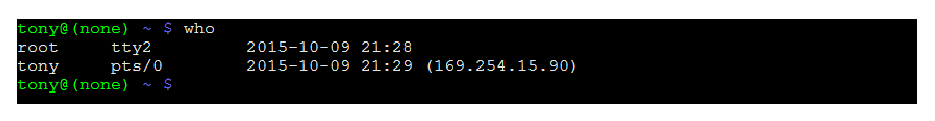
\includegraphics[width=15.5cm]{i03866x10.eps}$$

Here we see two users logged in: one named {\tt root} and the other named {\tt tony}.  The green text preceding each command-line prompt tells us who we are ({\tt tony}).  If we had any doubt, we could issue the command {\tt whoami} which will reply back with {\it our} user name.

\vskip 10pt

The {\tt root} user is sometimes called the {\it super-user} because of their unlimited privileges.  The {\tt root} user can delete or edit any file, in any directory, at any time.  As far as the Linux operating system is concerned, {\tt root} is God.  Therein lies a lesson: never sign into a Linux system as {\tt root} unless you are absolutely, one hundred percent sure of what you are doing.

\vskip 10pt

The text {\tt tty2} tells us that the {\tt root} user is logged into the system at a keyboard that is directly plugged into the Raspberry Pi computer.  ``{\tt tty}'' comes from the old days of {\it teletype} machines which were the equivalent of modern computer keyboards.  The text {\tt pts/0} (which stands for ``pseudo terminal slave'') tells us that the user ({\tt tony}) is logged into the system through a {\it network} connection.  The four dot-separated numbers shown in parentheses ({\tt 169.254.15.90}) shows the IP network address of the other computer from which {\tt tony} is logging in.

You will probably do most of your work on the caSCADA system via network connection to your own personal computer.  Free software is available for your download that lets any Microsoft Windows PC remotely log into any Linux computer using the {\it SSH} (Secure SHell) protocol.  This detail will be discussed later in this document.

\vskip 10pt

All the work you will be doing on the caSCADA system will be through the user account {\tt btc} (password also {\tt btc}).  This account will already be set up for you on each RTU's Raspberry Pi computer.



\vfil \eject

\vbox{\hrule \hbox{\strut \vrule{} {\tt ps} \vrule} \hrule} 

Linux is also a {\it multi-tasking} operating system, like Microsoft Windows.  This means it has the ability to execute multiple programs at once.  Single-processor computers manage this feat by switching attention really fast between all the running programs, giving the illusion that they're all running simultaneously.

\vskip 10pt

Each running program is called a {\it process} (not to be confused with the term ``process'' as it applies to industrial instrumentation).  Any user may view running processes on a Linux system by invoking the {\tt ps} command, although this command (without any options) doesn't provide much information.

\vskip 10pt

\vbox{\hrule \hbox{\strut \vrule{} {\tt ps -e} \vrule} \hrule} 

If we run the command {\tt ps -e} we will see a very long list of {\it every} process running in the operating system, including the {\tt ps} command itself:

$$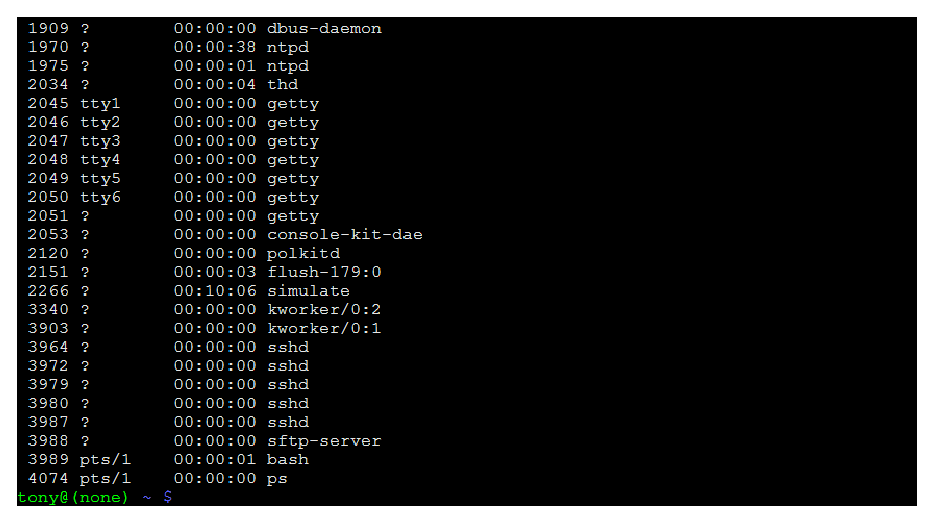
\includegraphics[width=15.5cm]{i03866x11.eps}$$

The list shown here is so long that it doesn't even fit the whole screen!

\vskip 10pt

\vbox{\hrule \hbox{\strut \vrule{} {\tt ps -u} {\it username} \vrule} \hrule} 

A more useful invocation of the {\tt ps} command shows us all the processes that have been run under a specified user name.  Here, we will view all the processes running under the user name {\tt tony} by entering the command as {\tt ps -u tony} (using the {\tt -u} ``user'' option):

$$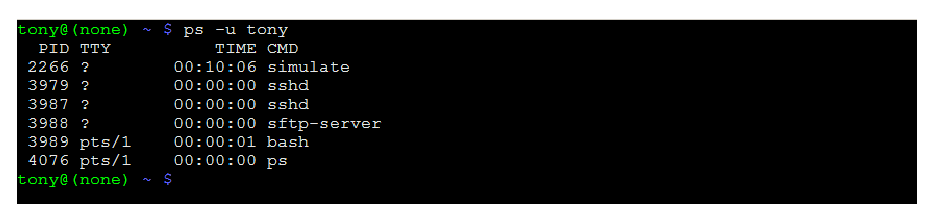
\includegraphics[width=15.5cm]{i03866x12.eps}$$

Each line displayed by the {\tt ps} command begins with a number, which is the {\it Process ID number}, or {\it PID} (not to be confused with ``PID'' control for industrial instrumentation!).  This number will become very useful to us for the next command.




\vfil \eject

\vbox{\hrule \hbox{\strut \vrule{} {\tt kill} \vrule} \hrule} 

From time to time it may be necessary for a user to halt a running process, especially one that runs without a live user interface.  This is done using the {\tt kill} command, which works by specifying the process ID number (PID) of the process you wish to terminate.

\vskip 10pt

The following illustration shows how to kill a running process called {\tt simulate}, which happens to be one of the processes used in the caSCADA telemetry system.  First, we see the {\tt ps} command being used to list all the processes started by the user {\tt tony} so we can identify its PID, then the {\tt kill} command being invoked to halt that one process, then the {\tt ps} command used again to prove the {\tt simulate} process is no longer running:

$$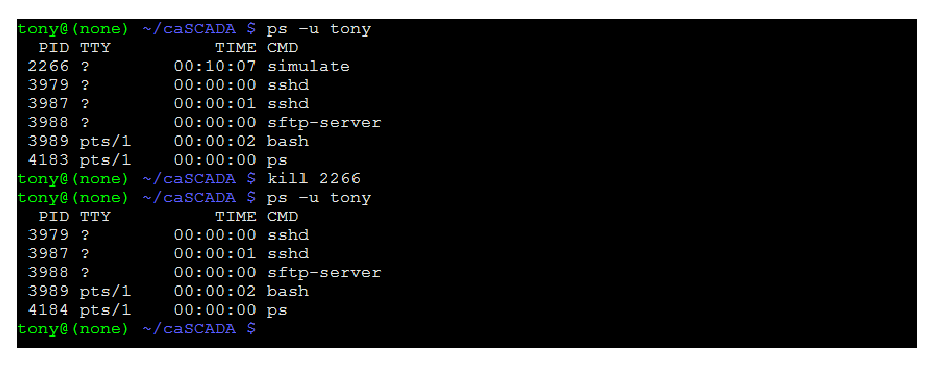
\includegraphics[width=15.5cm]{i03866x13.eps}$$

You will be doing this many times as you work with the caSCADA system, because processes such as {\tt simulate} run in the ``background'' (i.e. they don't prompt the user for any input, nor do they report any information to the command-line display).  When you make changes to the caSCADA software, you will need to ``compile'' those edits into an executable file that Linux can run, kill the version of that program currently running, and start up your newly modified version.

\vskip 20pt

As part of this lab exercise you will be asked to demonstrate the use of several of these commands, to ensure you are fluent enough in their use to work with the caSCADA system.









\vfil \eject

\noindent
{\bf Editing and running caSCADA code}

\vskip 5pt

The caSCADA system has been developed for the express purpose of teaching students how to write their own programming code in the C computer language, while at the same time building a working telemetry (SCADA) system measuring real-world data.

Each student team will be given a different piece of the caSCADA software (called a {\it function}) to modify for their own purposes.  Each team's function resides in its own file ending with the extension {\tt .c} which identifies it as a source code file written in the C language.  Students will use a text editor to modify their source file, then they will use another program in the Linux operating system called a {\it compiler} to translate that source code into instructions that Linux can directly execute.  After that, they will run their compiled program and monitor how well it performs the intended task.

\vskip 10pt

Like much of the software found on Linux (including all the essential parts of the Linux operating system itself), caSCADA is an {\it open-source} project.  This means all the source code files are available for perusal and modification.  This is very different from most of the software that Microsoft Windows users are familiar with, which is generally ``closed'' and therefore cannot be modified by the end-user.

Most open-source software projects provide a text file called {\tt README} or {\tt README.txt} describing details about the project.  caSCADA is no exception to this rule: in the {\tt caSCADA} directory you will find such a file describing how the system works, complete with examples of how to modify the function code to perform practical conditioning on real-world data.

\vskip 10pt

Here is a step-by-step summary of your program development cycle:

\begin{itemize}
\item{$(1)$} Use a text editor (e.g. {\tt nano}) to modify the source file for the channel you've been assigned.  For example, if you are assigned caSCADA channel number 6, then you will need to edit the file named {\tt f\_channel\_06.c} and then save those changes before exiting the text editor.
\vskip 5pt
\item{$(2)$} Next, re-compile the executable file by issuing a {\tt make} command followed by the name of the executable you wish to create.  The {\tt make} command invokes the compiler software for you, handling a bunch of technical details along the way, to make this task simpler.  You have only two options here: either run {\tt make poll} to compile the executable called {\tt poll} which gathers real data from the LabJack DAQ unit, or run {\tt make simulate} to compile the executable called {\tt simulate} which generates random data (useful in the absence of a LabJack DAQ) for your function to process.
\vskip 5pt
\item{$(3)$} Use the {\tt ps} command to check for currently-running instances of the executable.  If your user name is {\it btc}, for example, you will want to run {\tt ps -u btc}.  If one or more are running, halt them using the {\tt kill} command.  {\it There should never be more than one of {\tt poll} or {\tt simulate} running at any given time, and neither should you have {\tt poll} and {\tt simulate} running at once -- just one or the other, that's all!}
\vskip 5pt
\item{$(4)$} Start up a new instance of that process by typing the name of the executable (either {\tt poll} or {\tt simulate} depending on what you want to do) preceded by {\tt ./} and followed by an ampersand symbol ({\tt \&}).  For example, if you just compiled the {\tt simulate} executable file, you would run it by typing {\tt ./simulate \&} at the command prompt.  To run the {\tt poll} executable, type {\tt ./poll \&} at the command prompt.  Remember, you only need {\it one} of these running at any given time.  Running multiple instances of {\tt poll} and/or {\tt simulate} will write possibly conflicting data to the data files.
\vskip 5pt
\item{$(5)$} Read the contents of the {\tt data.txt} file to see how the data is being displayed.  I recommend typing {\tt cat data.txt} to do this.  If a console-based web browser such as {\tt lynx} is installed in the Linux computer, you may alternatively use it to view the contents of the {\tt data.html} file which will produce results that are better-formatted for easier viewing than the plain text file.  Both the {\tt poll} and the {\tt simulate} process updates both data files with fresh values once per second.  If everything is working as planned, you're done!  If not, go back to step 1 to fix your function and repeat all these steps.
\end{itemize}


\vfil \eject

You will find the caSCADA channel functions to be fairly easy to understand, even if you have never done any computer programming before.  For example, here is a listing of the default code for the source file {\tt f\_channel\_10.c}:

\vskip 10pt

\hbox{ \vrule
\vbox{ \hrule \vskip 3pt
\hbox{ \hskip 3pt
\vbox{ \hsize=6in \raggedright

{\tt /**********************************************************}

{\tt Consult the "README.txt" file for help editing this function!}

{\tt **********************************************************/}

\vskip 10pt

{\tt \#include <stdio.h>}

{\tt \#include <math.h>	    // Necessary for any advanced math functions}

{\tt \#include "cascada.h"  // Contains all the declarations specific to caSCADA}

\vskip 10pt

{\tt int}

{\tt f\_channel\_10 (void)}

$\lbrace$

\vskip 10pt

\hskip 10pt {\tt  f\_channel[10].value = ain[10];}

\hskip 10pt {\tt  f\_channel[10].tag = "(none)";}

\hskip 10pt {\tt  f\_channel[10].unit = "Volts";}

\hskip 10pt {\tt  f\_channel[10].status = 1;}

\hskip 10pt {\tt  f\_channel[10].comment = "Analog input AIN10";}

\vskip 10pt

\hskip 10pt {\tt return 1;}

$\rbrace$

}
\hskip 3pt}%
\vskip 5pt \hrule}%
\vrule}

\vskip 10pt

The only code you'll have to edit here is what falls between the curly brace characters ($\lbrace$ and $\rbrace$): that is to say, the lines of code assigning values to each element of the {\tt f\_channel[10]} data structure.  The first of these lines assigns {\tt f\_channel[10].value} to be equal to analog input 10 on the LabJack.  If AIN10 on the LabJack happens to measure 4.307 volts, then this function will place the number 4.307 into the variable {\tt f\_channel[10].value} where it will be displayed in the {\tt data.txt} file (and also in HTML format within another file named {\tt data.html}.  The lines assigning text (between quotation marks) to the {\tt .tag}, {\tt .unit}, and {\tt .comment} elements are for free-form text.  The {\tt .status} element is normally set to a value of 1 (which means ``good'' status), but may be set to other values at your discretion.

\vskip 10pt

You are welcome to make your function code as simple or as sophisticated as you desire.  Multiple examples are shown in the {\tt README.txt} file located with the other source files on the Raspberry Pi.  The following code segment shows a simple version of the {\tt f\_channel\_10.c} source file written to scale analog input number 3's 1-to-5-volt DC signal into a pressure measurement range of 0 to 75 PSI using a $y = mx + b$ equation where $m = 18.75$ and $b = -18.75$:

\vskip 10pt

\hbox{ \vrule
\vbox{ \hrule \vskip 3pt
\hbox{ \hskip 3pt
\vbox{ \hsize=6in \raggedright

{\tt int}

{\tt f\_channel\_10 (void)}

$\lbrace$

\vskip 10pt

\hskip 10pt {\tt  f\_channel[10].value = (ain[3] * 18.75) - 18.75;}

\hskip 10pt {\tt  f\_channel[10].tag = "PT-42";}

\hskip 10pt {\tt  f\_channel[10].unit = "PSI";}

\hskip 10pt {\tt  f\_channel[10].status = 1;}

\hskip 10pt {\tt  f\_channel[10].comment = "Receiver tank pressure";}

\vskip 10pt

\hskip 10pt {\tt return 1;}

$\rbrace$

}
\hskip 3pt}%
\vskip 5pt \hrule}%
\vrule}

\filbreak

\vskip 10pt

A good way for each student on a team to get experience programming a novel mathematical function without having to re-range their team's transmitter each time is to re-program the function for a different unit of temperature measurement on the exact same calibrated range.  For example, one student programs caSCADA to read out in degrees F, another in degrees C, another in degrees Rankine, and another in Kelvin, but each and every one of these uses the exact same calibrated range that the transmitter has been configured for.  This objective could even be checked by the instructor at the same time as the RTD or thermocouple simulation objective, with the student applying a simulated RTD/thermocouple signal to the transmitter and showing that simulated temperature displayed in a unique unit on the caSCADA display (i.e. the contents of the live {\tt data.txt} or {\tt data.html} file.

\vskip 10pt

If you would like to learn more about the mathematical and algorithmic capabilities offered by the C programming language, an excellent resource is the book {\it The C Programming Language} written by the inventors of C: Brian W. Kernighan and Dennis M. Ritchie.  Many other C programming tutorials and references may be found on the internet as well.  Suffice it to say, you can program each function to do almost {\it anything} to and with the channel data.  You may even program your function to read the values, statuses, and text fields of other channels, since all the channel variables are ``global'' and therefore accessible to all portions of the caSCADA software.

\vskip 10pt

C is a professional-grade programming language, which means that although the caSCADA system was written for use as a student learning system, anyone wishing to extend the capabilities of caSCADA beyond its intended use is welcome and able to do so because the C language is sufficiently capable for practically any task.  The fact that caSCADA is an {\it open-source} software project means anyone has the freedom to sample the C programming code and modify it to their heart's content without the need to request permission from the original developer.  This is the real beauty of open-source software: it gives you both the right and the means to {\it learn} from the code and {\it extend} that code well beyond its original intent.







\vfil \eject

\noindent
{\bf Lab questions}

\vskip 5pt

\begin{itemize}
\item{} {\bf Instrument connections}
\item{} Determine correct wire connections between instruments to create a working 4-20 mA loop circuit, based on diagrams of instruments with terminals labeled
\item{} Correctly determine all electrical sources and loads, as well as all voltage polarities and current directions in a 4-20 mA loop circuit, based on diagrams of instruments with terminals labeled
\end{itemize}

\filbreak

\begin{itemize}
\item{} {\bf Commissioning and Documentation}
\item{} Identify color codes and wire metals for a type J thermocouple
\item{} Identify color codes and wire metals for a type K thermocouple
\item{} Identify color codes and wire metals for a type T thermocouple
\item{} Identify color codes and wire metals for a type S thermocouple
\item{} Identify color codes and wire metals for a type E thermocouple
\item{} Rank types J, K, T, S, and E thermocouples according to their maximum temperatures
\item{} Explain what {\it cold-junction} (or {\it reference junction}) compensation is and why it is necessary
\item{} Explain how to distinguish thermocouple-grade wire from extension-grade wire
\end{itemize}

\filbreak

\begin{itemize}
\item{} {\bf Mental math} (no calculator allowed!)
\item{} Write a mathematical function to scale a temperature transmitter's signal into engineering units (e.g. degrees C or F) suitable for display in a SCADA system.
\end{itemize}

\filbreak

\begin{itemize}
\item{} {\bf Diagnostics}
\item{} Determine whether or not a given diagnostic test will provide useful information, given a set of symptoms exhibited by a failed system
\item{} Identify at least two plausible faults given the results of a diagnostic test and a set of symptoms exhibited by a failed system
\item{} Propose a diagnostic test for troubleshooting a failed system and then explain the meanings of two different test results
\end{itemize}



\underbar{file i03866}
%(END_QUESTION)





%(BEGIN_ANSWER)


%(END_ANSWER)





%(BEGIN_NOTES)

\vfil \eject


\noindent
{\bf Lab questions}

\vskip 20pt

\item{$(1)$} Sketch the necessary wire connections to build a working temperature-measurement loop, where the transmitter sends a signal to analog input AIN2 of the LabJack data acquisition unit.  Include any necessary components that are not already shown in this illustration:

\vskip 30pt

$$\includegraphics[width=15.5cm]{i03866x15.eps}$$

\vskip 20pt

\item{$(2)$} Identify color codes and wire metals for a {\it type T} thermocouple. 

\vskip 20pt

\item{$(3)$} Write a mathematical function capable of scaling a 1-5 VDC analog signal into a temperature range of 200 to 500 degrees Celsius.  Feel free to represent the analog signal value as $x$ and the scaled temperature value as $y$.

\vskip 20pt

\item{$(4)$} An indicating recorder with a thermocouple input (i.e. where the thermocouple connects directly to the recorder with no 4-20 mA transmitter in between) and a measurement range of $-100$ $^{o}$F to 900 $^{o}$F is registering 935 $^{o}$F, which the operator believes is unreasonable for this process.  Would shorting the recorder's two thermocouple connection screw terminals together with a jumper wire be a useful diagnostic test?  Explain why or why not.


\vfil \eject




\noindent
{\bf Lab questions}

\vskip 20pt

\item{$(1)$} Sketch the necessary wire connections to build a working temperature-measurement loop, where the transmitter sends a signal to analog input AIN1 of the LabJack data acquisition unit.  Include any necessary components that are not already shown in this illustration:

\vskip 30pt

$$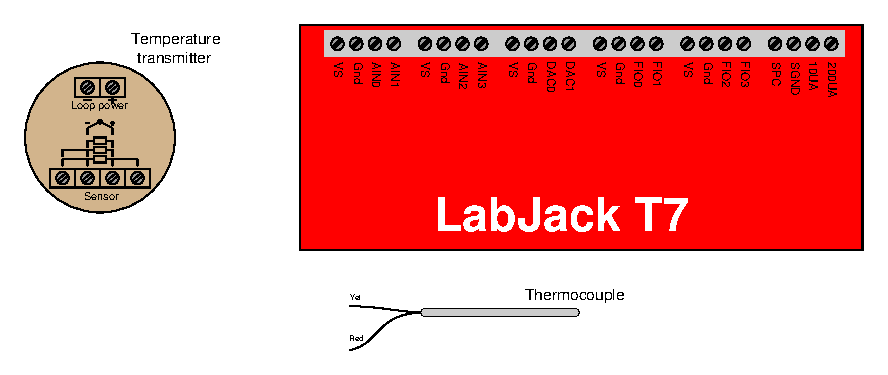
\includegraphics[width=15.5cm]{i03866x16.eps}$$

\vskip 20pt

\item{$(2)$} Identify color codes and wire metals for a {\it type J} thermocouple. 

\vskip 20pt

\item{$(3)$} Write a mathematical function capable of scaling a 1-5 VDC analog signal into a temperature range of 100 to 300 degrees Fahrenheit.  Feel free to represent the analog signal value as $x$ and the scaled temperature value as $y$.

\vskip 20pt

\item{$(4)$} An indicating recorder with an RTD input (i.e. where the 2-wire RTD connects directly to the recorder with no 4-20 mA transmitter in between) and a measurement range of 250 $^{o}$F to 450 $^{o}$F is registering 216 $^{o}$F, which the operator believes is unreasonable for this process.  Would shorting the recorder's two RTD connection screw terminals together with a jumper wire be a useful diagnostic test?  Explain why or why not.










%INDEX% Lab exercise, C programming
%INDEX% Lab exercise, Linux-based embedded system
%INDEX% Lab exercise, temperature measurement loop in caSCADA RTU node

%(END_NOTES)


